\chapter{PRBS modelling and implementation of pole-placement controller}
The aim of this chapter is to do PRBS testing on Single Board Heater System by the application of PRBS signal and also desing a pole-placement controller. The target group is anyone who has basic knowledge of Control Engineering. We have used Scilab with Xcos as an interface for sending and receiving data. This interface is shown in figure \ref{prbs-xcos}. Heater current and Fan speed are the two inputs to the system. The Heater current is varied with a PRBS signal. A provision is made to set the parameters like PRBS amplitude and offset value. A provision is also made to time the occurance of the PRBS input, using a step block. The value of step time in the step block has to be choosen carefully. Sufficient amount of time should be given to allow the temperature to reach a steady-state before the PRBS signal is applied. In this experiment we are keeping the Fan speed constant at 50\%. The temperature profile thus obtained is the output.

The first half of this chapter is dedicated to do system identification of the SBHS system using the response obtained for a PRBS (Pseudo Random Binary Sequence) input. In the second half, a pole-placement controller is designed using this model and implemented on SBHS.
\begin{figure}
\centering
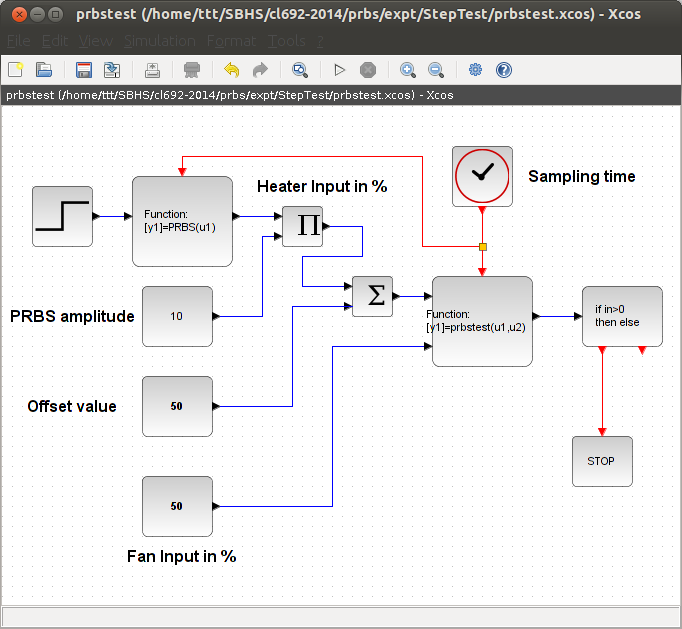
\includegraphics[width=0.7\linewidth]{prbs/prbs-xcos.png}
\caption{Xcos for PRBS testing experiment}
\label{prbs-xcos}
\end{figure}

\section{Issues with step testing and alternate approach}

SBHS is an example of a heater. Suppose you are working in a full scale plant. Current control system designed to control one of the heaters of the plant is lousy and your supervisor asked you to design a new controller from scratch. The first step you need to do is identification of the heater transfer function. The catch is, plant is currently
operational. You can't shut the plant down to identify the heater transfer function. You have to do it while the heater is operating in the plant. You might think of giving the heater a positive step and measuring the response in the controlled temperature. This will
increase the temperature of the component being heated for the period of time step is applied. However, if the process is sensitive to temperature of the component (distillation, for example), it will go off the desired course and the output of the whole plant will be affected and will be undesirable.

\vspace{12pt}

There is an alternate approach which is widely used in industry. The input given to the heater for identification is not step, but a \textbf{pseudo-random binary sequence (PRBS)}. The concept behind PRBS is that the input is perturbated in such a way that the time average of the input is the value at which it is being operated currently. Thus, some positive and some negative steps can be given. This results some positive and some negative changes in the temperature which leads to the time average of the performance of the plant remaining the same. Thus, PRBS testing can be done in a working plant without affecting the plant performance unlike step testing. A typical PRBS and corresponding plant output looks like as shown in figure \ref{sample-prbs}

\begin{figure}[H]
\begin{centering}
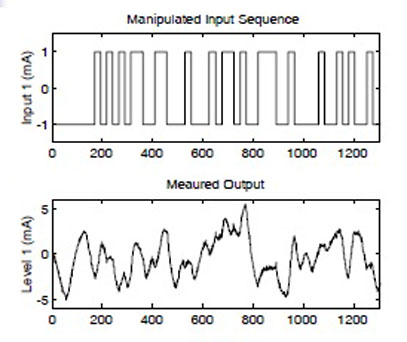
\includegraphics[width=0.6\textwidth]{prbs/PRBS}
\par\end{centering}

\caption{PRBS testing input and output \textit{{[}Image source: CL 686 Advanced
Process Control, Spring 2013-14 lecture slides. Prof. S. C. Patwardhan, IIT Bombay{]}}}
\label{sample-prbs}
\end{figure}


\section{Step by step procedure to do PRBS testing}

Similar to Chapter \ref{chap1} and \ref{chap2}, in this section we will find the transfer function model of SBHS. But there are two major differences. First difference is that we will give a Pseudo Random Binary Sequence to the heater input of SBHS and second difference is that we will find the discrete time transfer function. A Pseudo Random Binary Sequence is nothing but a signal whose amplitude varies between two limits randomly at any given time. An illustration of the same is given in figure \ref{prbs-fig}. A PRBS signal can be easily generated using the $rand()$ function in scilab. Scilab code to generate the PRBS signal is given at the end of this chapter. Figure \ref{prbs-xcos} shows the xcos diagram for PRBS testing. The PRBS amplitude and offset value to the input can be adjusted using the relevant blocks. 

The steps to be followed to conduct PRBS test experiment remains same as explained in section \ref{linux_scilab} for linux users and section \ref{scilab_sbhs} for windows users. The only difference is that the prbs experiment function is written in {\tt prbstest.sci} file and the xcos is saved in file {\tt prbstest.xcos}. These files should be used for doing prbs experiment. The PRBS response obtained after executing the experiment successfully is shown in figure \ref{prbs-res}
\begin{figure}
\centering
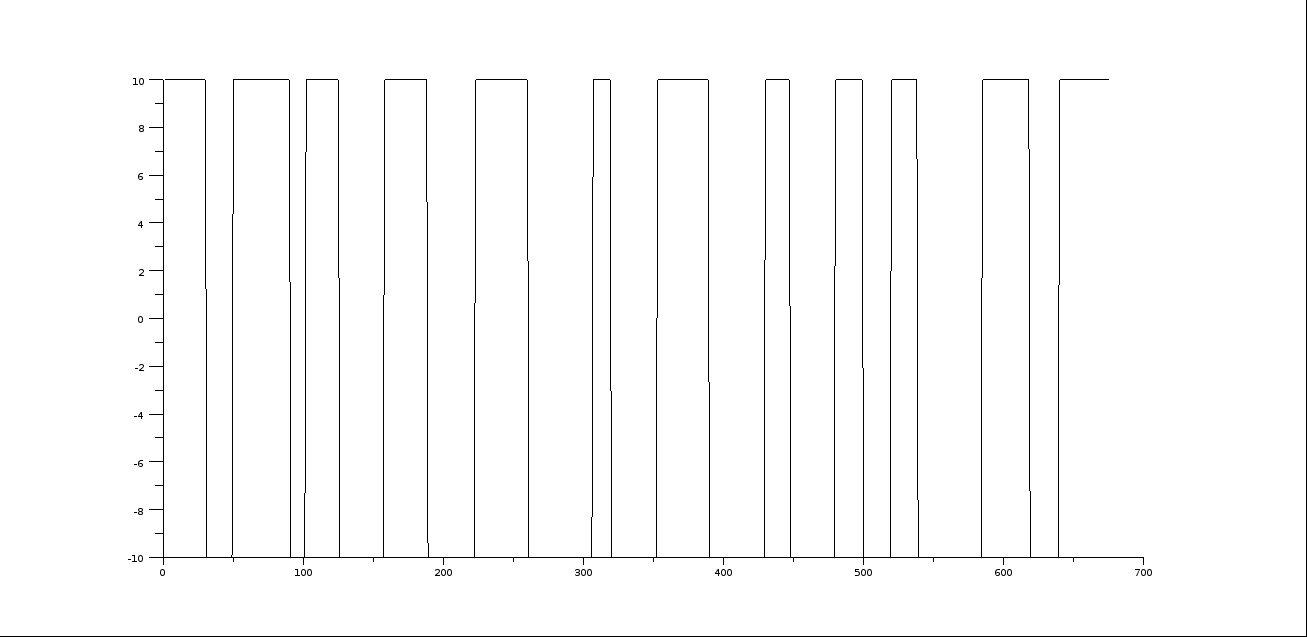
\includegraphics[width=0.7\linewidth]{prbs/prbs-illustration.png}
\caption{A Pseudo Random Binary Sequence}
\label{prbs-fig}
\end{figure}

\begin{figure}
\centering
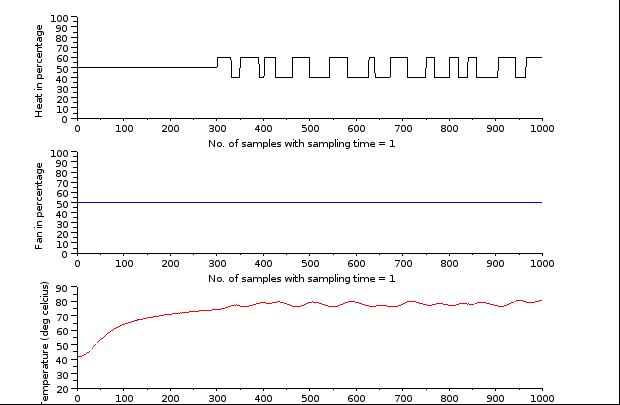
\includegraphics[width=0.7\linewidth]{prbs/prbs-expt.png}
\caption{PRBS testing response}
\label{prbs-res}
\end{figure}


\section{Determination of discrete time transfer function}

System identification is carried out to identify the transfer function between the input signal to the system and output from the system. Firstly a transfer function with unknown parameters is assumed. The system is given a known input and its response is obtained and then the values of the unknown parameters is chosen such that the sum of squares of the errors is minimized. Here, the error is the difference between the actual output and the output predicted by the transfer function model assumed.



For the given SBHS system, we assume a second order transfer function:

\begin{align}\label{DTF}
G(z)=\frac{b_{1}+b_{2}z^{-1}}{1+a_{1}z^{-1}+a_{2}z^{-2}}z^{-d}
\end{align}


The unknown parameters $a_1, a_2, b_1, b_2$ and d are to be obtained through the response of the system to the known inputs.  $a_1, a_2, b_1, b_2$ are real numbers and d is the plant delay which is an integer.  For these model parameters estimation, we used a pseudo random binary sequence (PRBS) input. Since the optimization over discrete variables (d in this case) is a very difficult routine for computers, we assume a value of d and then optimize over  $a_1, a_2, b_1, b_2$. The optimization problem, then, becomes:


\begin{align}
(\hat{b_1}, \hat{b_2}, \hat{a_1}, \hat{a_2})=\underset{b_1, b_2, a_1, a_2}{argmin}\sum_{i=0}^{N}(y(k)-\hat{y}(k))^{2}
\end{align}


Here, $y(k)$ is the output obtained from the system, so it is known, $\hat{y(k)}$ is the estimated output using $y$ the model assumed, which can be written as a difference equation:

\begin{align}
\hat{y}(k) = -a_1\hat{y}(k - 1) - a_2\hat{y}(k - 2) + b_1 u(k - d) + b_2 u(k - 1 - d)
\end{align}

The optimization is performed using the optimization routine “optim” of Scilab. Copy the  data file to the folder {\tt prbs\_analysis}. Change the scilab working directory to {\tt prbs\_analysis} folder. Open the file {\tt optimize.sce} and put the name of the data file (with extention) in the filename field. Save and run this code and obtain the plot as shown in figure 4.3. This code uses the routines {\tt label.sci}, {\tt costfunction.sci} and {\tt second\_order.sci}. This code will give optimized values for $a_1, a_2, b_1, b_2$ which can be used to define a second order discrete time transfer function as given in equation \ref{DTF}. The results generated after executing optimization routine over the data file obtained earlier is shown in figure \ref{prbs-fit} and figure \ref{prbs-model}. The initial values were choosen to be [0.5 0.5 0.5 0.5]. The value of $err$ along with the fit obtained has to be used to change the initial values and the value of $delay$ The transfer function thus obtained is 

\begin{align}\label{model}
G(z)=\frac{0.0022266 - 0.0017656 z^{-1}}{1-1.912876z^{-1}+0.9162750z^{-2}}z^{-d}
\end{align}


\begin{figure}
\centering
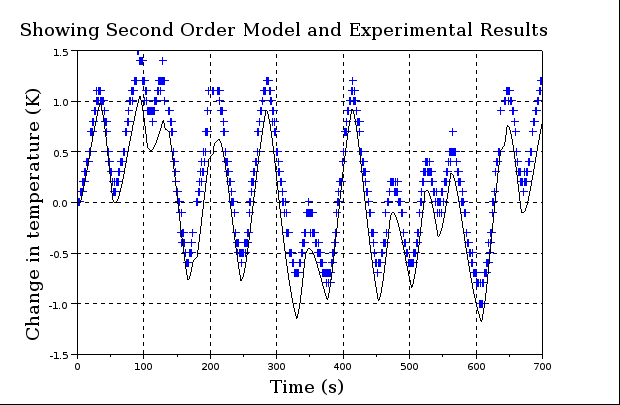
\includegraphics[width=0.7\linewidth]{prbs/prbs-fit.png}
\caption{PRBS testing response}
\label{prbs-fit}
\end{figure}

\begin{figure}
\centering
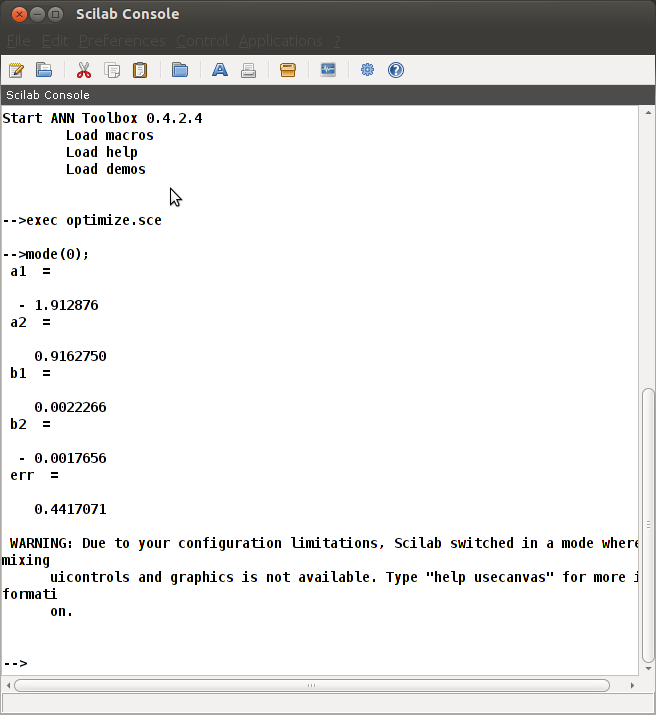
\includegraphics[width=0.7\linewidth]{prbs/prbs-model.png}
\caption{PRBS testing response}
\label{prbs-model}
\end{figure}



\subsection{Performing PRBS testing on SBHS, virtually}
The step by step procedure for conducting an experiment virtually is explained in section \ref{vlabsexpt}. The required .sce file is {\tt prbstest.sce}.  You will find this file in the {\tt prbs} directory under {\tt virtual} folder. The necessary codes are listed in the section \ref{prbscodes}


\section{Scilab Code}\label{prbscodes}
\begin{code}
\ccaption{ser\_init.sce}{\ttfamily ser\_init.sce}
\lstinputlisting{Scilab/local/imc_controller/ser_init.sce}
\end{code}

\begin{code}
 \ccaption{imc.sci}{\ttfamily imc.sci}
\lstinputlisting{Scilab/local/imc_controller/imc.sci}
\end{code}


\begin{code}
 \ccaption{imc\_virtual.sce}{\ttfamily imc\_virtual.sce}
\lstinputlisting{Scilab/virtual/imc_controller/imc_virtual.sce}
\end{code}


\begin{code}
 \ccaption{imc\_virtual.sci}{\ttfamily imc\_virtual.sci}
\lstinputlisting{Scilab/virtual/imc_controller/imc_virtual.sci}
\end{code}


%\bibliography{imc} 
